\section{Results of BADA 4 implementation}
This section presents the validation and analysis of the results obtained from implementing \gls{apm}s based on pyBADA libraries into BlueSky and migrating the existing kinematic-based model to a dynamic approach. With the intention of isolating the effect of the \gls{apm}, all the simulations presented in this section were conducted under \gls{isa} conditions.

Although BlueSky already has BADA 3 compatibility, this functionality has been migrated to use the pyBADA libraries. Parallel to this migration, a full implementation of the BADA 4 model has been developed, not available in the simulator until now. This new architecture enables uniform access to the various BADA model families and facilitates the incorporation of more advanced formulas for aircraft performance calculations. 

Beyond incorporating new data models, integrating pyBADA has required revising the internal mechanisms used to calculate relevant magnitudes, such as available thrust, drag, and fuel flow. This has allowed obtaining a more truthful representation of the aircraft behaviour. 

The main goal of this analysis is to determine up to what point the implementation of BADA 4 and the migration of BADA 3 improves physical consistency and simulator fidelity when compared to BlueSky's base configuration. Special attention is paid to trajectory generation, behaviour during climb and descent, engine thrust modelling, and fuel flow estimation.

The following subsections present the verification of the correct implementation of the models based on pyBADA and, next, the impact these changes have on the simulated aircraft and on the overall fidelity of the simulation.

\subsection{Migration of the aircraft performance framework to pyBADA}
The original BlueSky simulator includes a built-in BADA 3 performance model based on direct lookups in tables and simplified analytic expressions derived from BADA 3 user manual. Although it is functional for basic trajectory simulations, this implementation does not make use of the official BADA libraries and depend on a set of static data kept locally that is not updated with the newer BADA versions. Furthermore, it does not expose the full set of physical magnitudes defined by the BADA specification, such as the energy share factor (ESF), the reduced climb power coefficient, or the aerodynamic configuration state.

The migration described in this thesis replaces the original BlueSky's performance engine with a plugin-based architecture built on top of the pyBADA library, the official implementation in Python distributed by EUROCONTROL alongside BADA datasets. This library provides structured access to \gls{apm} data for both BADA 3 and BADA 4 and implements equations corresponding to the \gls{tem} in a validated and version-controlled codebase.

The new architecture is implemented as a single, unified BlueSky simulation plugin named \texttt{DYNAMIC\_BADA} (\texttt{dynamic\_bada/plugin.py}). This plugin consolidates all pyBADA-based performance computation into a multi-fidelity framework controlled by a per-aircraft fidelity parameter. Rather than maintaining separate plugins for kinematic and dynamic performance models, \texttt{DYNAMIC\_BADA} exposes three fidelity modes via the \texttt{DYNMODE} stack command:

\begin{itemize}
    \item \textbf{MODE~0} (Kinematic): Full pyBADA force, fuel flow, mass, and phase computation every tick. The vertical speed and longitudinal acceleration are \emph{not} overridden, so BlueSky's kinematic autopilot continues to drive the trajectory. This mode produces output identical to a standalone kinematic performance observer and is the baseline for validation.
    \item \textbf{MODE~1} (Point-mass dynamic): MODE~0 performance computation plus trajectory overrides. The rate of climb or descent (ROCD) computed from the pyBADA energy equation is written back to \texttt{bs.traf.vs[i]}, and the longitudinal acceleration from the force balance is written back to \texttt{bs.traf.ax[i]}. BlueSky's kinematic autopilot still manages heading. This is the default mode.
    \item \textbf{MODE~2} (Coupled dynamic): MODE~1 plus lateral-longitudinal coupling. Roll dynamics track the commanded bank angle at a configurable roll rate. The load factor $n = 1/\cos\phi$ is applied, turn-induced drag via $C_{L,\text{turn}} = n \cdot C_{L,\text{level}}$ feeds the drag polar, and heading is integrated from $\dot{\psi} = g \tan\phi / V_{\text{TAS}}$.
\end{itemize}

The BADA generation (BADA~3.15 or BADA~4.2) is independently selectable via the \texttt{DYNBADA} stack command, either globally or per aircraft, without restarting the simulation.

This plugin inherits from \texttt{PerfBase}, the abstract performance interface defined by BlueSky, and the three mandatory methods are overwritten: \texttt{create()}, \texttt{update()}, and \texttt{limits()}. This design ensures total compatibility with the rest of the simulator without modifying any source-code file from BlueSky.

A model-caching mechanism is implemented in the plugin to avoid redundant file reads: once a \texttt{Bada3Aircraft} or \texttt{Bada4Aircraft} object is instantiated for a given aircraft type, the reference is stored in a dictionary (\texttt{cached models}) and reused for every posterior aircraft of the same type within the same simulation run. This substantially reduces the initialisation computational effort in multi-aircraft scenarios.

When an aircraft model is not found in the available BADA dataset, the plugin applies a fallback strategy: in BADA 4, the generic Dummy-TWIN model is used. And in BADA 3, the closest available entry is selected by the pyBADA library itself. For both cases, the slot is flagged as \texttt{is\_dummy = True}, which is later used to adjust the flight envelope enforcement logic, as detailed in section 3.2.5.

\subsubsection{Plugin architecture and integration verification}
The \texttt{DYNAMIC\_BADA} plugin was created by subclassing BlueSky's core performance interface, \texttt{PerfBase}. Internally, the plugin delegates aircraft creation, per-tick state updates, and envelope-limit enforcement to a unified adapter layer (\texttt{BadaInterface}) that abstracts both BADA~3.15 and BADA~4.2. The active BADA generation can be switched at runtime via the stack command \texttt{DYNBADA 3|4}, allowing direct comparison of both datasets within a single simulation session. The fidelity mode is independently controlled via \texttt{DYNMODE 0|1|2}, either globally or per aircraft. The architecture of this integration is shown in Figure~3.1, while the per-tick update loop is detailed in Figure~3.2.


\begin{figure}[H]
    \centering
    \includegraphics[width=0.65\linewidth]{Flowchart_plugin_1_sec3_2.png}
    \caption{Plugin software architecture}
    \label{fig:placeholder}
\end{figure}

\begin{figure}[H]
    \centering
    \includegraphics[width=0.65\linewidth]{Flowchart_plugin_2_sec3_2_2.png}
    \caption{Per-tick \texttt{update()} flowchart}
    \label{fig:placeholder}
\end{figure}


\paragraph{Passive observer integration model (MODE~0).}
An important architectural characteristic of \texttt{DYNAMIC\_BADA} in MODE~0 is that it operates as a \emph{passive performance observer}. Under BlueSky's standard plugin architecture, subclasses of \texttt{PerfBase} are responsible for calculating performance coefficients (such as current thrust, drag, fuel flow, and maximum speed/altitude limits) but do not control the numerical integration of the aircraft's state vector. 

At each simulation tick of duration $\Delta t$, the plugin runs the full pyBADA pipeline: atmospheric state evaluation, aerodynamic force computation, flight phase detection, thrust rating selection, fuel flow calculation, and mass depletion. However, in MODE~0 these computed values for vertical speed and longitudinal acceleration are not written back to BlueSky's core state vectors (such as \texttt{bs.traf.vs[i]} for vertical speed or \texttt{bs.traf.ax[i]} for longitudinal acceleration). Instead, they are stored in internal arrays for logging purposes (e.g., via the \texttt{SAVEHEADER} plugin). BlueSky's internal kinematic autopilot continues to update the aircraft's position, altitude, and speed independently based on simple geometric and kinematic relationships. The pyBADA-derived limits only affect the trajectory indirectly by clipping the autopilot commands through the \texttt{limits()} hook.

This architecture is fundamental to the validation methodology presented in this section: MODE~0 allows direct comparison of pyBADA's performance outputs (thrust, drag, fuel flow, mass) against external references while maintaining an identical trajectory generation mechanism across all BlueSky-based configurations.

\paragraph{Dynamic trajectory override model (MODE~1 and MODE~2).}
In contrast to MODE~0, fidelity modes 1 and 2 actively write computed state overrides back into BlueSky's traffic arrays. In MODE~1, the rate of climb or descent derived from the pyBADA energy equation replaces the kinematic autopilot's commanded vertical speed during Climb and Descent phases, and the longitudinal acceleration from the force balance $a_x = (T - D - W \sin\gamma) / m$ replaces the autopilot's speed-error correction. A monkey-patched version of \texttt{Traffic.update\_airspeed} ensures that, for MODE~1 and MODE~2 aircraft, the true airspeed (TAS) is integrated from the force-balance acceleration rather than the autopilot's proportional speed-error signal. MODE~2 extends this further by introducing roll dynamics, load-factor coupling, and heading integration from the coordinated-turn equation.

The fidelity mode can be changed at any point during the simulation via the \texttt{DYNMODE} command, either globally (\texttt{DYNMODE 1}) or per aircraft (\texttt{DYNMODE acid 2}). This enables comparative studies in which the same scenario is executed under different fidelity assumptions without requiring separate simulation runs.

\paragraph{AT-speed waypoint semantics.}
The plugin monkey-patches two BlueSky autopilot methods --- \texttt{Autopilot.wppassingcheck} and \texttt{Route.direct} --- to enforce AT-speed waypoint semantics. In the unmodified BlueSky autopilot, waypoint speed constraints are treated as advisory targets that the autopilot may or may not reach by the time the waypoint is passed. The patched versions ensure that, upon passing a waypoint with a speed constraint, the autopilot immediately adopts the constrained speed as the active target. This is essential for realistic simulation of published SID/STAR speed schedules, where speed constraints at specific waypoints are mandatory.

\paragraph{Mathematical formulation of the update loop.}
At each tick, the plugin computes the aircraft's performance using standard BADA formulations. These computations are executed regardless of the fidelity mode; the mode only determines which of the resulting quantities are written back to BlueSky's state vectors:
\begin{enumerate}
    \item \textbf{Atmospheric properties}: Local pressure $P$ and temperature $T_{\text{atm}}$ are read from BlueSky, and the dimensionless atmospheric ratios are computed:
    \begin{equation}
        \theta = \frac{T_{\text{atm}}}{T_0}, \quad \delta = \frac{P}{P_0}, \quad \sigma = \frac{\delta}{\theta}
    \end{equation}
    where $T_0 = 288.15$\,K and $P_0 = 101{,}325$\,Pa are the ISA sea-level references. The local speed of sound is $a = a_0 \sqrt{\theta}$ (with $a_0 = 340.294$\,m/s), and the Mach number is $M = V / a$.
    
    \item \textbf{Aerodynamic forces}: The lift coefficient $C_L$ is computed assuming wings-level, quasi-steady flight where lift balances weight ($L = W = m \cdot g_0$):
    \begin{equation}
        C_L = \frac{2 \, m \, g_0}{\sigma \, \rho_0 \, V^2 \, S}
    \end{equation}
    where $g_0 = 9.80665$\,m/s\textsuperscript{2}, $\rho_0 = 1.225$\,kg/m\textsuperscript{3} is the sea-level air density, and $S$ is the wing reference area. The drag coefficient $C_D$ is evaluated using the BADA aerodynamic polar for the current configuration (Climb, Cruise, or Descent):
    \begin{equation}
        C_D = C_{D_0} + C_{D_2} \cdot C_L^2
    \end{equation}
    The total aerodynamic drag force is then:
    \begin{equation}
        D = \frac{1}{2} \sigma \, \rho_0 \, V^2 \, S \, C_D
    \end{equation}
    
    \item \textbf{Thrust rating selection}: Engine thrust $T$ is computed based on the detected flight phase:
    \begin{itemize}
        \item \emph{Climb}: Operated at full maximum climb thrust ($T_{\max}$ under MCMB rating): $T = T_{\max}$. The BADA~3 User Manual defines a reduced climb power coefficient $C_{\text{cr}}$ to account for lower-than-MTOW operations; however, this reduction is not applied in the current implementation — full MCMB thrust is always commanded during climb.
        \item \emph{Descent}: Operated at descent thrust (LIDL rating). In BADA~3, $T = \max(T_{\text{des}}, T_{\text{idle}})$ is computed as a logged performance value; in BADA~4, $T = T_{\text{idle}}$. In MODE~0 this thrust value is recorded for fuel flow computation but does not control the geometric autopilot's vertical speed. In MODE~1 and MODE~2, the resulting ROCD from the energy equation is written back to the trajectory integrator.
        \item \emph{Cruise}: Computed as the thrust required to balance drag and acceleration ($T = D + m \cdot a_x$), clamped between idle thrust and maximum cruise thrust ($T_{\text{mcrz}}$). To prevent algebraic loops, the acceleration $a_x$ from the previous tick is used.
    \end{itemize}
    
    \item \textbf{Rate of climb or descent (ROCD)}: The vertical speed is computed from the Total Energy Model:
    \begin{equation}
        \text{ROCD} = \frac{(T - D) \cdot V}{m \, g_0} \cdot \text{ESF}, \quad
        \text{ESF} = \left[ 1 + \frac{V}{g_0} \frac{\mathrm{d}V}{\mathrm{d}h} \right]^{-1}
        \label{eq:rocd_tem}
    \end{equation}
    In MODE~0, this ROCD value is computed and logged but not written back to \texttt{bs.traf.vs[i]}; the kinematic autopilot's geometric vertical speed prevails. In MODE~1 and MODE~2, the ROCD is written back to the trajectory integrator during the Climb and Descent phases, making the vertical profile physically consistent with the force balance.

    \item \textbf{Longitudinal acceleration}: The net longitudinal acceleration is computed from Newton's second law along the flight-path axis:
    \begin{equation}
        a_x = \frac{T - D - W \sin\gamma}{m}
        \label{eq:ax_force_balance}
    \end{equation}
    where $\gamma = \arcsin(VS / V_{\text{TAS}})$ is the flight-path angle. In MODE~0, this value is logged but not applied; in MODE~1 and MODE~2, it replaces the autopilot's proportional speed-error correction.

    \item \textbf{Fuel flow and mass depletion}: Fuel flow $FF$ (in kg/s) is queried from the pyBADA engine model as a function of the computed thrust, current speed, altitude, and configuration. The aircraft mass is then decremented for the next tick:
    \begin{equation}
        m_{t+\Delta t} = m_t - FF \cdot \Delta t
        \label{eq:mass_depletion}
    \end{equation}
    This mass depletion is applied in all fidelity modes (0, 1, and 2), ensuring that fuel consumption is always tracked regardless of whether the trajectory is kinematically or dynamically driven.
\end{enumerate}

To avoid the computational overhead of reloading aircraft XML datasets from disk on every aircraft creation, the plugin implements a cached model dictionary (\texttt{cachedmodels}). In a scenario containing multiple aircraft of the same type, only the first instantiation triggers a disk read. Posterior creations retrieve the cached reference in less than $1$\,ms.

When the requested aircraft type is not found in the local BADA database, a fallback mechanism is triggered. The BADA~4 sub-model falls back to the generic \texttt{Dummy-TWIN} model (hard-coded as the class constant \texttt{FALLBACK\_TYPE}), while the BADA~3 sub-model loads a generic aircraft from the DUMMY data directory (the exact resolved type depends on the installed dataset). In both cases, the aircraft slot is flagged with \texttt{is\_dummy~=~True}. This flag disables the altitude ceiling check in \texttt{limits()}, in order to prevent the dummy's artificially low ceiling from constraining the simulation, while still enforcing the speed envelope ($V_{\min}$, $V_{\max}$) to avoid unphysical speed spikes.

\subsubsection{Stack commands and runtime control}
\label{sec:stack_commands}

The \texttt{DYNAMIC\_BADA} plugin exposes five stack commands that allow the user to configure and inspect the performance model at runtime without restarting the simulation:

\begin{itemize}
    \item \texttt{DYNMODE [acid] <0|1|2>}: Sets the fidelity mode globally (if no aircraft identifier is provided) or for a specific aircraft. For example, \texttt{DYNMODE 0} configures all aircraft to MODE~0 (kinematic), while \texttt{DYNMODE KLM123 2} sets only the aircraft \texttt{KLM123} to MODE~2 (coupled dynamic). The fidelity mode can be changed at any point during the simulation.

    \item \texttt{DYNBADA [acid] <3|4>}: Selects the BADA generation (BADA~3.15 or BADA~4.2) globally or per aircraft. This command triggers a re-initialisation of the underlying \texttt{BadaInterface} for the affected aircraft, loading the corresponding aerodynamic and engine model from the pyBADA library.

    \item \texttt{MASS acid <mass\_kg>}: Overrides the operating mass of the specified aircraft immediately at the moment the command is executed. The new mass value (in kilograms) replaces the current mass in the performance model's internal array and is used from the very next simulation tick onward; fuel burn continues to be decremented from this updated value. This command is particularly useful for initialising aircraft at a specific operating mass that differs from the default reference mass provided by the BADA dataset, or for simulating in-flight mass changes due to payload drops or aerial refuelling. The command enforces a plausibility guard: mass values below $500$\,kg or above $1{,}000{,}000$\,kg are rejected with a warning, preventing accidental unit errors (e.g., entering mass in tonnes rather than kilograms).

    \item \texttt{DYNSTATS acid}: Displays the full dynamic state of a specific aircraft, including the current fidelity mode, BADA generation, flight phase, thrust, drag, fuel flow, mass, and all internal state-machine variables. This command is intended for debugging and real-time monitoring during development.

    \item \texttt{DYNRESET}: Re-reads the plugin's \texttt{config.yaml} configuration file without restarting the simulation. This allows runtime adjustment of parameters such as the default fidelity mode, BADA data directories, vertical speed thresholds, roll rate limits, and integration method.
\end{itemize}

\subsubsection{Flight phase detection algorithm}
\label{sec:phase_detection}
A critical requirement for realistic aircraft performance simulation is the accurate detection of flight phases (Climb, Cruise, and Descent), since the detected phase determines the thrust rating applied at each time step: maximum climb thrust (MCMB) during Climb, idle thrust (LIDL) during Descent, and a drag-balanced thrust clamped to the maximum cruise rating (MCRZ) during Cruise. If the phase detection algorithm is not properly developed, it will corrupt thrust, fuel flow, and the resulting trajectory.

Rather than relying on instantaneous vertical speed thresholding, which is highly sensitive to autopilot altitude captures and atmospheric turbulence, the \texttt{DYNAMIC\_BADA} plugin implements a dynamic, non-monotonic finite state machine with temporal persistence (hysteresis). This state machine is shared across all fidelity modes (0, 1, and 2); the detected phase determines the thrust rating and fuel flow computation identically regardless of whether the trajectory is kinematically or dynamically driven.

\paragraph{Phase detection criteria and threshold selection.}
The state machine evaluates three inputs at each time step: the aircraft's instantaneous vertical speed ($VS$), current pressure altitude ($h$), and the autopilot target altitude ($h_{\text{AP}}$). The transition criteria and their justification are:

\begin{itemize}
    \item \textbf{Altitude capture band} ($\Delta h_{\text{TOC}} = \Delta h_{\text{TOD}} = 500$\,ft). This parameter establishes a vertical window around the autopilot target altitude $h_{\text{AP}}$ (i.e., $|h - h_{\text{AP}}| \le 500$\,ft) that serves two purposes:
    \begin{itemize}
        \item \emph{Cruise Transition Gate}: As the aircraft climbs or descends towards $h_{\text{AP}}$, entering this band is a necessary condition to trigger the transition to the Cruise phase (signalling Top-of-Climb or Top-of-Descent/intermediate level-off).
        \item \emph{Step Maneuver Guard}: Cruising aircraft are locked into the Cruise phase until the autopilot target altitude $h_{\text{AP}}$ is set to a new target that deviates by more than $500$\,ft (i.e., $|\Delta h| > 500$\,ft). This prevents minor autopilot altitude tracking errors or atmospheric perturbations from triggering an unintended state change.
        \item \emph{Operational Rationale}: The $\pm 500$\,ft threshold matches typical VNAV control law capture bands and respects the Reduced Vertical Separation Minimum (RVSM) standard of $1{,}000$\,ft. Since adjacent flight levels in RVSM are separated by $1{,}000$\,ft, a $\pm 500$\,ft capture band ensures that an aircraft's stabilization zone never overlaps with adjacent flight levels.
    \end{itemize}

    \item \textbf{Vertical speed thresholds} ($VS_{\text{climb}} = +300$\,ft/min, $VS_{\text{descent}} = -300$\,ft/min, $VS_{\text{level}} = \pm 150$\,ft/min). Instantaneous vertical speed ($VS$) is highly susceptible to high-frequency noise from atmospheric turbulence and autopilot pitch corrections. These thresholds introduce a hysteresis mechanism to ensure robust phase transitions:
    \begin{itemize}
        \item \emph{Level-flight stabilization} ($VS_{\text{level}}$): A strict threshold of $\pm 150$\,ft/min ensures the aircraft has physically stabilized and stopped its vertical rate before Cruise is declared. The transition to Cruise requires the aircraft to stay within both the altitude capture band and the $VS_{\text{level}}$ band.
        \item \emph{Maneuver confirmation} ($VS_{\text{climb}}$ / $VS_{\text{descent}}$): The wider thresholds of $+300$\,ft/min (for active climbs/re-climbs) and $-300$\,ft/min (for active descents/re-descents) exceed the typical vertical speed noise floor observed in BlueSky cruise flight ($\pm 50$ to $200$\,ft/min). This prevents momentary atmospheric fluctuations or autopilot adjustments from triggering spurious Climb or Descent phase declarations.
    \end{itemize}
    
    \item \textbf{Minimum cruise altitude} ($h_{\min,\text{cruise}} = 10{,}000$\,ft). Standard instrument departure (SID) procedures frequently impose intermediate altitude constraints below 10,000\,ft. If the state machine were allowed to declare Cruise at these low altitudes, the engine model would switch from maximum climb thrust to cruise thrust prematurely, resulting in an unrealistic climb. This threshold ensures the Climb phase is maintained throughout the departure segment.
\end{itemize}
\begin{figure}[H]
    \centering
    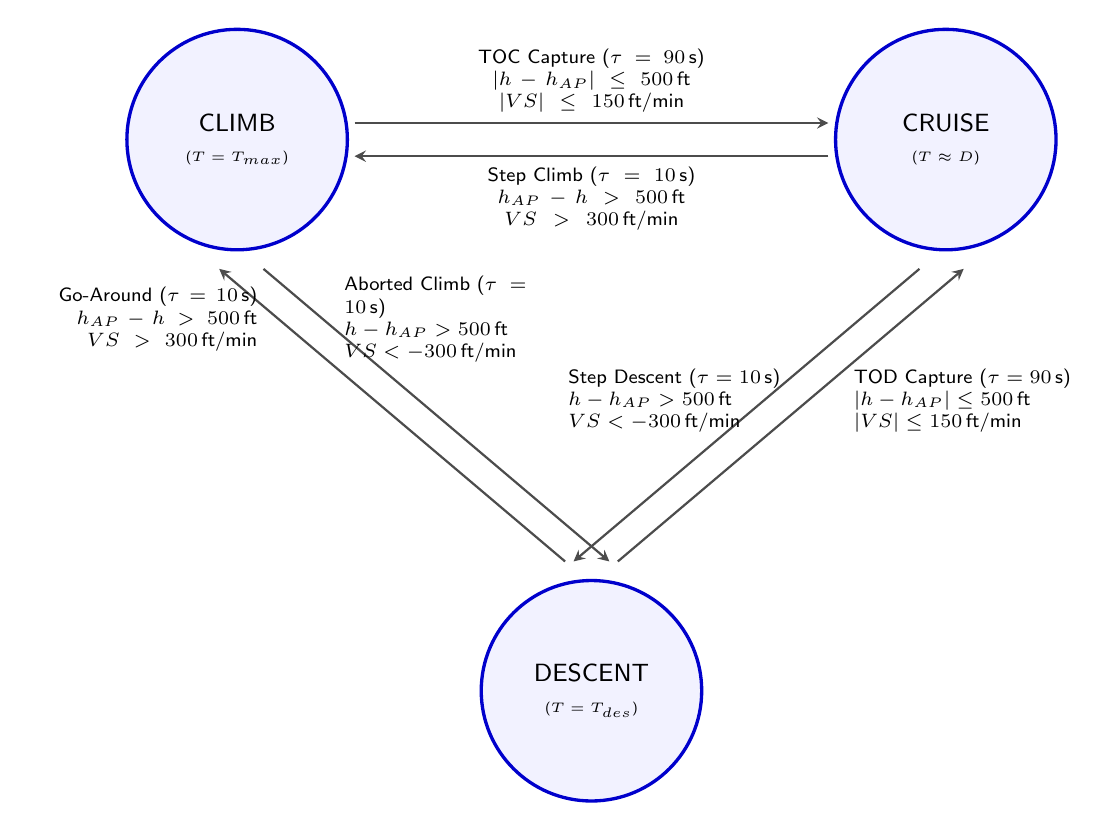
\begin{tikzpicture}[
        state/.style={circle, draw=blue!80!black, fill=blue!5, very thick,
                      minimum size=2.8cm, align=center, font=\sffamily\small},
        transition/.style={->, >=stealth, shorten >=2pt, shorten <=2pt, thick,
                           draw=black!70, align=center, font=\sffamily\scriptsize}
    ]
        % --- Nodes ---
        \node[state] (climb)   at (0,  0)  {CLIMB \\ \tiny ($T = T_{\text{max}}$)};
        \node[state] (cruise)  at (9,  0)  {CRUISE \\ \tiny ($T \approx D$)};
        \node[state] (descent) at (4.5,-7) {DESCENT \\ \tiny ($T = T_{\text{des}}$)};

        % -------------------------------------------------------
        % CLIMB <-> CRUISE  (horizontal)
        % -------------------------------------------------------
        \draw[transition]
            ([yshift=6pt]climb.east) -- ([yshift=6pt]cruise.west)
            node[above, midway, text width=3.8cm, align=center] {
                TOC Capture ($\tau=90$\,s)\\
                $|h-h_{\text{AP}}|\le500$\,ft\\
                $|VS|\le150$\,ft/min
            };

        \draw[transition]
            ([yshift=-6pt]cruise.west) -- ([yshift=-6pt]climb.east)
            node[below, midway, text width=3.8cm, align=center] {
                Step Climb ($\tau=10$\,s)\\
                $h_{\text{AP}}-h>500$\,ft\\
                $VS>300$\,ft/min
            };

        % -------------------------------------------------------
        % CLIMB <-> DESCENT
        % -------------------------------------------------------

        % DESCENT -> CLIMB  (Go-Around): label near CLIMB end
        \draw[transition]
            ([xshift=-8pt, yshift=5pt]descent.north)
            -- ([xshift=-8pt, yshift=-5pt]climb.south)
            node[left, pos=0.82, text width=2.8cm, align=right, xshift=-4pt] {
                Go-Around ($\tau=10$\,s)\\
                $h_{\text{AP}}-h>500$\,ft\\
                $VS>300$\,ft/min
            };

        % CLIMB -> DESCENT  (Aborted Climb): label near CLIMB end
        \draw[transition]
            ([xshift=8pt, yshift=-5pt]climb.south)
            -- ([xshift=8pt, yshift=5pt]descent.north)
            node[right, pos=0.18, text width=2.8cm, align=left, xshift=4pt] {
                Aborted Climb ($\tau=10$\,s)\\
                $h-h_{\text{AP}}>500$\,ft\\
                $VS<-300$\,ft/min
            };

        % -------------------------------------------------------
        % CRUISE <-> DESCENT
        % -------------------------------------------------------

        % DESCENT -> CRUISE  (TOD Capture): shifted right and up
        \draw[transition]
            ([xshift=8pt, yshift=5pt]descent.north)
            -- ([xshift=8pt, yshift=-5pt]cruise.south)
            node[right, pos=0.18, text width=2.8cm, align=left,
                 xshift=60pt, yshift=40pt] {
                TOD Capture ($\tau=90$\,s)\\
                $|h-h_{\text{AP}}|\le500$\,ft\\
                $|VS|\le150$\,ft/min
            };

        % CRUISE -> DESCENT  (Step Descent): shifted right and up
        \draw[transition]
            ([xshift=-8pt, yshift=-5pt]cruise.south)
            -- ([xshift=-8pt, yshift=5pt]descent.north)
            node[left, pos=0.82, text width=2.8cm, align=left,
                 xshift=60pt, yshift=40pt] {
                Step Descent ($\tau=10$\,s)\\
                $h-h_{\text{AP}}>500$\,ft\\
                $VS<-300$\,ft/min
            };

    \end{tikzpicture}
    \caption{Flight phase detection state transition diagram. Edges list the
             transition criteria (altitude differences and vertical speed thresholds)
             and the required persistence duration~($\tau$).}
    \label{fig:phase_detection_fsm}
\end{figure}

\paragraph{Temporal persistence filter.}
To prevent high-frequency oscillations (chatter) between states, particularly during the altitude capture manoeuvre, where the autopilot may overshoot and cause the vertical speed to cross the level-flight threshold multiple times, the state machine applies a temporal accumulator filter. Two per-aircraft variables are maintained: a candidate state $s_{\text{cand}}$ and a transition timer $t_{\text{accum}}$. At each simulation tick of duration $\Delta t$:

\begin{enumerate}
    \item If the trigger criteria for a new candidate phase $s_{\text{cand}} \neq s_{\text{current}}$ are met and $s_{\text{cand}}$ is the same as in the previous tick, the timer is incremented: $t_{\text{accum}} \leftarrow t_{\text{accum}} + \Delta t$.
    \item If $s_{\text{cand}}$ differs from the previous tick's candidate, the timer is reset: $t_{\text{accum}} \leftarrow \Delta t$.
    \item The transition is executed only when $t_{\text{accum}} \geq \tau_{\text{threshold}}$.
    \item If no transition condition is met, both $t_{\text{accum}}$ and $s_{\text{cand}}$ are reset.
\end{enumerate}

The threshold values $\tau$ are asymmetric by design:

\begin{itemize}
    \item \textbf{Active phase transitions} ($\tau = 10$\,s, \texttt{TRANSITION\_ACCUM\_THRESHOLD}). Transitions from Cruise into Climb or Descent must be fast: a $10$-second delay ensures that maximum climb thrust (MCMB) or idle descent thrust (LIDL) is engaged promptly when a step climb or descent is initiated, avoiding the aircraft climbing sluggishly under cruise power.

    \item \textbf{Cruise phase transitions} ($\tau = 90$\,s, \texttt{CRUISE\_ACCUM\_THRESHOLD}). Transitions into Cruise require a much longer confirmation window. During altitude capture, autopilot controllers exhibit damped oscillations that typically settle within 30--60\,seconds. The $90$-second timer acts as a low-pass filter, delaying the Cruise declaration until the aircraft has fully stabilised. This prevents erratic switching between full-climb thrust and cruise thrust coefficients ($C_t$) during capture, which would cause unrealistic thrust and fuel flow spikes.
\end{itemize}

\paragraph{Step climb and step descent support.}
Unlike strictly monotonic phase models (where the sequence Climb~$\rightarrow$~Cruise~$\rightarrow$~Descent is irreversible), the non-monotonic design permits backward transitions. This is essential for realistic en-route operations:

\begin{itemize}
    \item \textbf{Step Climb (SC):} If the aircraft is in Cruise and the autopilot commands a higher altitude ($h_{\text{AP}} - h > 500$\,ft and $VS > 300$\,ft/min), the state machine transitions back to Climb after $10$\,seconds, allowing a new climb segment at full MCMB thrust.

    \item \textbf{Step Descent (SD):} If the aircraft is descending and levels off at an intermediate flight level (above $10{,}000$\,ft, within $\pm 500$\,ft of the autopilot target, $|VS| \leq 150$\,ft/min), the state machine transitions to Cruise after $90$\,seconds. When the autopilot subsequently commands a lower altitude, the state machine transitions back to Descent after $10$\,seconds.

    \item \textbf{Go-around / Re-climb:} From the Descent phase, a transition to Climb is triggered if $VS > 300$\,ft/min and $h_{\text{AP}} - h > 500$\,ft, modelling emergency go-around or missed approach procedures.
\end{itemize}

\subsubsection{Assumptions and constraints}
The implementation and validation of the \texttt{DYNAMIC\_BADA} plugin are subject to several technical and physical assumptions, as well as operational constraints:

\begin{itemize}
    \item \textbf{Performance Model Fallbacks due to Licensing}: In the absence of complete, licensed BADA datasets for specific aircraft types, the dispatcher falls back to generic representatives (\texttt{J2M} for BADA~3 and \texttt{Dummy-TWIN} for BADA~4). Under this fallback state, the altitude ceiling constraint is disabled to prevent unphysical constraints on en-route cruise profiles, while the speed envelopes are still enforced. Consequently, performance metrics (such as fuel flow and climb rates) for fallback aircraft reflect generic twin-engine characteristics rather than type-specific performance.
    
    \item \textbf{Instantaneous Engine Response}: During the Cruise phase, the thrust required is computed algebraically using the force balance $T = D + m \cdot a_x$ and clamped between $T_{\text{idle}}$ and $T_{\text{mcrz}}$. This assumes that the engine can adjust its thrust instantaneously to match drag and longitudinal acceleration. No transient throttle response times, spool-up/spool-down delays, or rotor dynamics are modeled.
    
    \item \textbf{Autopilot Target Dependence}: The flight phase detection algorithm relies heavily on the autopilot target altitude ($h_{\text{AP}}$) as a proxy for operational intent. If $h_{\text{AP}}$ is undefined or is not set ahead of a maneuver, the state machine defaults to the current pressure altitude, which may delay or prevent the transition between Climb, Cruise, and Descent phases.
    
    \item \textbf{Minimum Cruise Altitude Constraint}: A hard constraint of $h_{\min,\text{cruise}} = 10{,}000$\,ft is enforced to prevent the state machine from entering the Cruise phase during intermediate altitude holds on SIDs. While appropriate for commercial operations, this constraint prevents the realistic simulation of low-altitude cruise profiles for turboprops, general aviation, or short-haul flights.
    
    \item \textbf{Atmospheric and Wind Assumptions}: The BADA Total Energy Model (TEM) equations assume quasi-steady, symmetric flight in a standard atmosphere. The validation campaign is conducted under International Standard Atmosphere (ISA) conditions with zero wind. The introduction of wind gradients, turbulence, or severe temperature deviations in a full simulation would affect the Energy Share Factor (ESF) and resulting rate of climb/descent calculations.
    
    \item \textbf{Three-Degrees-of-Freedom (3-DOF) Point-Mass Model}: Consistent with BADA's underlying framework, the aircraft is modeled as a point mass in MODE~0 and MODE~1. Aerodynamic forces are resolved along the velocity vector, and rotational dynamics (pitch, roll, and yaw) are neglected. MODE~2 extends this to include roll dynamics and load-factor coupling, but pitch and yaw dynamics remain unmodelled.

    \item \textbf{Fidelity mode equivalence in MODE~0}: The validation results presented in this section were obtained using MODE~0, which produces performance outputs (thrust, drag, fuel flow, mass, and phase) identical to those of a standalone kinematic performance observer. The trajectory in MODE~0 is driven entirely by BlueSky's geometric kinematic autopilot; the pyBADA-computed ROCD and longitudinal acceleration are logged but not applied. This must be taken into account when interpreting vertical profile and speed comparisons, as explained in Sections~3.2.4 and~3.2.5.
\end{itemize}

\subsubsection{Simulation setup and comparison methodology}
To evaluate the accuracy and consistency of the \texttt{DYNAMIC\_BADA} plugin in MODE~0, a validation campaign was designed comprising 27~flight scenarios covering a representative sample of European commercial routes. Each scenario defines a complete gate-to-gate flight with waypoint routes, altitude constraints, and speed targets derived from published SID/STAR procedures. All simulations were conducted under ISA (International Standard Atmosphere) conditions to isolate the effect of the performance model from meteorological variability.

\paragraph{Scenario classification.}
The 27 evaluation flights are selected from the standard flight testing suite to stress-test the plugin across distinct operational regimes and geographical constraints:
\begin{itemize}
    \item \textbf{Category 1: Domestic and Ultra-Short Flights:} High-frequency hop routes (e.g., LEIB $\rightarrow$ LEPA  or EGHI $\rightarrow$ EGJA ) characterized by very low cruise altitudes (FL040--FL180). These test rapid phase transitions and minimum cruise height filtering under conditions where a stable cruise phase is virtually non-existent.
    \item \textbf{Category 2: Major European Trunk Routes:} Standard medium-haul flights representing the baseline density of European airspace (e.g., LEBL $\rightarrow$ EGKK and EHAM $\rightarrow$ LIRF ). Operating between FL240 and FL410 , these provide stable cruise benchmarks and test Flight Information Region (FIR) transitions.
    \item \textbf{Category 3: Long-Haul Intra-European Flights:} Routes stretching between 3 and 6 hours over geographical boundaries (e.g., EFHK $\rightarrow$ GCTS). These are critical for analyzing long-duration deep cruise stability and the simulation of continuous fuel-weight reduction and associated step-climb profiles.
    \item \textbf{Category 4: Widebody Operations:} High-density or cargo repositioning flights utilizing heavy long-haul aircraft categories (A350) on short sectors (e.g., EGLL $\rightarrow$ EDDF). These focus on validating aerodynamics and engine performance envelopes for high-inertia aircraft at atypical low cruise altitudes.
    \item \textbf{Category 5: Complex Scenarios and Edge Cases:} Geographically demanding flight paths designed to challenge the limits of the plugin. This includes steep initial climb profiles out of high-altitude alpine terrain (LOWI), severe oceanic windshear and remote overwater tracking (LPMA), entry into Eurocontrol space from third-country boundaries (GMMN), and transoceanic oceanic control zones (BIKF).
\end{itemize}

\todo{add plot of all the flight routes}

Each of the 27~scenarios was executed under four different performance configurations, yielding a total of $27 \times 4 = 108$ simulation runs:

\begin{table}[H]
\centering
\caption{Performance model configurations compared.}
\label{tab:models_compared}
\begin{tabular}{llll}
\hline
\textbf{Label} & \textbf{Source} & \textbf{Backend} \\
\hline
BlueSky (base) & Built-in BlueSky performance model & BADA 3 \\
BADA 3 (pyBADA) & \texttt{DYNAMIC\_BADA}, DYNMODE~0, \texttt{DYNBADA~3} & pyBADA 3.15 \\
BADA 4 (pyBADA) & \texttt{DYNAMIC\_BADA}, DYNMODE~0, \texttt{DYNBADA~4} & pyBADA 4.2 \\
Dynamo & External trajectory simulation tool & University tool \\
\hline
\end{tabular}
\end{table}
The Dynamo simulator is an independent high-fidelity trajectory computation tool developed at the university that serves as the ground-truth reference in this study. It was run under identical ISA atmospheric conditions and waypoint routes as the BlueSky simulations, and its outputs are treated as the closest available approximation to real aircraft behaviour.


\paragraph{Implementation differences between BlueSky BADA~3 and pyBADA BADA~3.}
\label{par:bada3_impl_diff}
Although both the \emph{BlueSky (base)} and \emph{BADA~3 (pyBADA)} configurations use the same BADA~3.15 aerodynamic dataset (OPF/APF coefficient files), their numerical implementations differ substantially across five dimensions. These differences are the principal reason why the two BADA~3 variants do not produce identical results, and understanding them is essential for interpreting the comparison.
\begin{enumerate}
    \item \textbf{Flight phase detection algorithm.} The BlueSky built-in BADA~3 implementation uses a six-phase, instantaneous speed- and altitude-threshold state machine (phases: TO, IC, CR, AP, LD, GD) driven by the current calibrated airspeed (CAS) and altitude relative to the autopilot target. Phase transitions are applied at each simulation tick without any temporal hysteresis. In contrast, the \texttt{DYNAMIC\_BADA}/pyBADA implementation uses a three-phase finite state machine (Climb, Cruise, Descent) with a temporal persistence filter: a transition into the Cruise phase requires a sustained 90-second stabilisation window within an altitude capture band of $\pm 500$\,ft and a vertical speed below $150$\,ft/min, while transitions from Cruise into Climb or Descent require a 10-second confirmation. This asymmetric hysteresis prevents spurious phase oscillations during altitude capture but delays the idle-thrust descent trigger relative to the BlueSky model, which may enter the approach (AP) or landing (LD) phase—and hence use lower thrust settings—earlier in the trajectory.

    \item \textbf{Climb thrust and reduced power coefficient.} The BADA~3 User Manual defines a \emph{reduced climb power} coefficient $C_{\text{red}}$ that limits maximum climb thrust below the nominal MCMB rating when the aircraft operates at a mass significantly lower than MTOW. The BlueSky implementation applies this coefficient during the entire sub-ceiling climb phase:
    \begin{equation}
        C_{\text{pred}} = 1 - C_{\text{red}} \cdot \frac{m_{\max} - m}{m_{\max} - m_{\min}}
    \end{equation}
    The \texttt{DYNAMIC\_BADA}/pyBADA BADA~3 sub-model does not apply this reduction — it always uses the full MCMB rating during climb. This means pyBADA systematically applies higher climb thrust than the BlueSky built-in, resulting in faster climbs, a higher Top-of-Climb thrust, and consequently higher fuel flow during the climb phase. This is a deliberate implementation choice in the plugin (the reduced power lines are present in the source code but are commented out), as the BlueSky autopilot's kinematic trajectory is not coupled back to the performance model's ROCD output.

    \item \textbf{Descent thrust computation.} The BlueSky native implementation computes descent thrust as a fraction of maximum climb thrust using phase- and altitude-dependent descent thrust coefficients from the BADA OPF file:
    \begin{equation}
        T_{\text{des}} = C_{t,\text{des,high}} \cdot T_{\max} \quad (h > H_{p,\text{des}}), \qquad
        T_{\text{des}} = C_{t,\text{des,low}} \cdot T_{\max} \quad (h \leq H_{p,\text{des}})
    \end{equation}
    The pyBADA implementation invokes the library method \texttt{ac.TDes()} and then clamps the result to a hard idle-thrust lower bound: $T = \max(T_{\text{des}}, T_{\text{idle}})$. In practice the coefficient-based formula in the BlueSky model can yield values below the idle floor for certain configurations, while the pyBADA clamp prevents this. In MODE~0, this thrust value is used exclusively for fuel flow computation and logging — it does not feed back into the autopilot's vertical speed, so it has no direct effect on the geometric descent trajectory. In MODE~1 and MODE~2, the resulting ROCD from the energy equation is written back to the trajectory integrator, producing a dynamically consistent descent profile.

    \item \textbf{Fuel flow formulation.} The BlueSky native implementation computes three separate fuel flow branches — nominal ($\eta \cdot T$), cruise-corrected ($\eta \cdot T \cdot C_{f,\text{cruise}}$), and minimum ($C_{f3}(1 - h/C_{f4})$) — and selects among them based on the current phase. The cruise fuel correction factor $C_{f,\text{cruise}}$ from the OPF file is applied only during level cruise segments. The pyBADA BADA~3 implementation delegates fuel flow computation entirely to the \texttt{ac.ff()} library method, which encapsulates phase, thrust, speed, and altitude in a single call. Differences in how the library internally applies $C_{f,\text{cruise}}$ and the minimum fuel flow floor lead to systematic fuel flow offsets, particularly during the transition between the climb and cruise phases.

    \item \textbf{Passive observer model and vertical speed coupling.} In MODE~0, both implementations ultimately rely on BlueSky's geometric kinematic autopilot to drive the trajectory. Neither computes ROCD from the Total Energy Model and writes it back to the trajectory integrator as a primary control signal. The native BADA~3 implementation does invoke \texttt{calclimits()}, which produces a thrust-saturation-limited vertical speed (\texttt{limvs}) passed back as \texttt{allowed\_vs}; however, this limit fires only when the commanded thrust exceeds the maximum available thrust (\texttt{Thr > maxthr - 1.0}), making it a climb saturation guard rather than a general ROCD controller. The \texttt{DYNAMIC\_BADA} plugin in MODE~0 provides no such mechanism: its \texttt{limits()} function returns \texttt{allow\_vs = intent\_vs} unchanged in all flight phases. The plugin therefore operates as a pure \emph{passive performance observer} in MODE~0 — computing thrust, drag, and fuel flow for logging and emission estimation, while leaving the vertical trajectory entirely in the hands of BlueSky's geometric autopilot. In MODE~1 and MODE~2, the computed ROCD is written back to the trajectory integrator, fundamentally changing this relationship.
\end{enumerate}

In summary, despite accessing the same BADA~3.15 coefficient database, the two BADA~3 configurations constitute fundamentally different implementations. The observed performance differences between \emph{BlueSky (base)} and \emph{BADA~3 (pyBADA)} in Sections~3.2.4--3.2.6 are therefore attributable to these algorithmic divergences, not to differences in the underlying aerodynamic data. This distinction is critical for a correct interpretation of the validation results.

For each simulation run, the following variables were recorded at each tick via the \texttt{SAVEHEADER} logging plugin: time~($t$), distance flown~($s$), altitude~($h$), TAS, CAS, Mach number, vertical speed~($VS$), thrust~($T$), throttle~($THR\%$), fuel flow~($FF$), aircraft mass~($m$), temperature~($T_{\text{atm}}$), and flight path angle~($\gamma$).

\paragraph{Error metrics.}
For each scenario~$k$ and each pair of models $(A, B)$, the per-flight deviation is computed by interpolating both trajectories onto a common distance grid and evaluating the mean absolute error (MAE) for a given variable~$x$:
\begin{equation}
    \text{MAE}_{k}(x) = \frac{1}{N_k} \sum_{j=1}^{N_k} \left| x_{A}(s_j) - x_{B}(s_j) \right|
\end{equation}
where $N_k$ is the number of sample points in scenario~$k$. The campaign-level metric is the average of these per-flight errors across all retained scenarios:
\begin{equation}
    \overline{\text{MAE}}(x) = \frac{1}{N_{\text{retained}}} \sum_{k=1}^{N_{\text{retained}}} \text{MAE}_{k}(x)
\end{equation}

Critically, both trajectories are interpolated onto a common fractional distance grid $\xi \in [0, 1]$, where $\xi = 0$ corresponds to departure and $\xi = 1$ to arrival. This normalisation is essential because the different simulators use different time references and distance conventions (Dynamo uses a destination-referenced negative distance, while BlueSky uses an origin-referenced positive distance), making direct time-domain comparison invalid. Only airborne data (altitude $h > 50$\,ft) is used in the interpolation to exclude taxi phases.

This approach captures not only the systematic bias between models but also the scenario-to-scenario variability of the deviations (e.g., whether discrepancies are concentrated in long-haul flights or short-range routes).

\paragraph{Outlier filtering and database fallbacks.}
To ensure the comparison is physically meaningful, an outlier filtering process was applied to the flight database. A flight was discarded from the comparison if any model's simulated range was less than $85\%$ of the reference Dynamo range (indicating premature simulation crash or termination) or if the TAS MAE between that model and Dynamo exceeded $100$\,kt.

Based on these criteria, only 1 of the 27 flights was identified as an outlier and excluded from the global statistics: \texttt{LEIB-LEPA}, due to a range shortfall where the simulated range in the base BlueSky BADA~3 model (102\,NM) was less than $85\%$ of the Dynamo reference range (123\,NM). All other flights completed the flight path successfully across all models.

Retaining the remaining 26 flights ensures that the comparison evaluates only valid simulations for which all models completed the flight path successfully.

\subsubsection{Vertical profile comparison}

The altitude and vertical speed profiles are visualised in Figure~\ref{fig:altitude_profiles} for a representative selection of routes. These profiles illustrate the fundamental kinematic differences between the four models across the three flight phases.

\paragraph{Climb phase.}
All four models show broadly consistent altitude profiles during the initial climb phase, reaching the assigned cruise flight level within a comparable distance. This is expected: both BADA~3 and BADA~4 apply maximum climb thrust (MCMB) during the climb phase, which forces the aircraft to follow the geometric altitude constraints of the waypoint route. The Dynamo reference also shows a typical commercial climb profile with a constant-CAS/constant-Mach speed schedule and a progressive altitude gain. Minor differences in the Top-of-Climb (TOC) distance arise from different fuel-mass feedback loops: in the pyBADA models, the aircraft mass continuously decreases due to fuel burn, reducing the thrust-to-weight ratio and slightly lengthening the climb. For a representative A320 flight (Munich--Stockholm, EDDM--ESSA, $774$\,NM), all models reach FL370 within approximately 15\% of total flight progress, consistent with standard commercial operating procedures.

\paragraph{Cruise phase.}
During cruise, the altitude profiles are nominally aligned across all models, as the autopilot holds the assigned flight level. The most significant kinematic differences in cruise are related to vertical speed oscillations: BlueSky's kinematic autopilot exhibits non-zero vertical speed residuals (of the order of $\pm 100$--$200$\,ft/min) due to proportional altitude control laws, whereas Dynamo maintains cruise altitude with sub-10\,ft/min precision. The pyBADA models fall between these extremes, with BADA~4 showing slightly smoother altitude tracking than BADA~3 due to its more refined thrust-clamping formulation during cruise. The global VS MAE across the entire flight is $311.31 \pm 311.41$\,ft/min for BlueSky, $303.77 \pm 295.03$\,ft/min for BADA~3, and $304.24 \pm 296.17$\,ft/min for BADA~4 (Figure~\ref{fig:mae_boxplots}). The comparable vertical speed errors across all models confirm that they share the same kinematic autopilot, with only minor differences arising from speed envelope transitions and differences in the detected flight phase triggers.

\paragraph{Descent phase.}
The descent phase is where the most significant structural difference in autopilot architecture between the four configurations manifests. It is important to clarify a key architectural constraint that applies to \emph{all three BlueSky-based configurations in MODE~0}: BlueSky's kinematic autopilot drives the trajectory in all cases. It projects the required altitude loss over the remaining waypoint distance to compute a commanded vertical speed, without applying any aerodynamic force balance. This means that none of the performance models in MODE~0 --- native BlueSky BADA~3, \texttt{DYNAMIC\_BADA} BADA~3, or \texttt{DYNAMIC\_BADA} BADA~4 --- compute ROCD from the Total Energy Model and write it back to the trajectory integrator.

The \texttt{DYNAMIC\_BADA} plugin in MODE~0 operates as a \emph{passive performance observer}, as explicitly established in Section~3.2.1. During the Descent phase, pyBADA selects idle thrust (LIDL rating) and computes the corresponding fuel flow for logging purposes, but this computed thrust value does not feed back into BlueSky's kinematic autopilot. The autopilot continues to determine the actual rate of descent geometrically from the waypoint altitude constraints. The native BlueSky BADA~3 implementation includes a thrust-saturation-limited vertical speed feedback via \texttt{calclimits()} (which fires only when thrust exceeds its maximum rating), but this is a climb-phase saturation guard, not a descent rate controller.

The differences in altitude profiles between models are therefore driven by two factors acting through the autopilot's \emph{speed} input, not its vertical speed input. First, the \texttt{DYNAMIC\_BADA} plugin enforces strict per-aircraft speed envelope limits (Vmin, Vmax, and the below-10{,}000\,ft limit of 250\,kt) via its \texttt{limits()} hook. Since the geometric autopilot computes the required descent gradient as a function of current speed, a lower commanded speed produces a shallower geometric descent slope. The native BlueSky BADA~3 model enforces a broader speed envelope that allows higher descent speeds. Second, the three-phase persistence-filter state machine in \texttt{DYNAMIC\_BADA} transitions to Descent (and the associated idle thrust computation) at a different point along the route than the six-phase instantaneous FSM in the native BADA~3 model, producing differences in the logged thrust and fuel flow profiles without directly affecting the trajectory shape.

The global altitude MAE values against Dynamo --- $611.83 \pm 596.81$\,ft for BlueSky (native), $669.34 \pm 640.52$\,ft for BADA~3 (pyBADA), and $671.89 \pm 643.29$\,ft for BADA~4 (pyBADA) --- primarily reflect the mismatch between BlueSky's geometric waypoint-following autopilot and Dynamo's VNAV-optimised trajectory computation, not differences between the performance models themselves. The slightly lower altitude MAE achieved by the native model is a geometric artefact: without speed envelope enforcement, the native model allows higher speeds and steeper descent gradients, which happen to match Dynamo's altitude profile more closely in the distance domain.


\subsubsection{Speed and envelope enforcement}

The TAS and Mach number profiles are shown in Figure~\ref{fig:speed_profiles}. These profiles reveal important differences in how each model enforces the operational speed envelope.

\paragraph{Speed limit enforcement.}
In the base BlueSky model, no maximum operational Mach limit is imposed during cruise. As a consequence, the autopilot commands whatever speed is kinematically consistent with the flight plan, frequently resulting in Mach numbers that exceed the maximum operating Mach ($M_{\text{mo}}$) of the aircraft. In the retained flights, BlueSky reaches mean maximum Mach values of $0.800$--$0.810$, with several flights briefly exceeding the representative $M_{\text{mo}} = 0.82$. While this Mach number is technically within limits, the absence of any physical enforcement mechanism means that this is purely scenario-dependent and would fail for tighter profiles.

The \texttt{DYNAMIC\_BADA} plugin enforces BADA's per-aircraft maximum and minimum speed envelope at every tick via the \texttt{limits()} hook. This clamps the Mach number at approximately $M = 0.82$ during cruise. Both pyBADA sub-models successfully enforce these bounds, which is confirmed by the fact that neither BADA~3 nor BADA~4 produces Mach values exceeding the representative $M_{\text{mo}}$ in any of the 26 retained flights. The Dynamo reference consistently produces cruise Mach values of $0.78$--$0.78$, reflecting its use of cost-index-based optimal cruise speeds that are typically below the maximum Mach limit.

\paragraph{Speed MAE analysis.}
The global TAS MAE across the 26 retained flights is $12.58 \pm 11.79$\,kt for BlueSky, $16.56 \pm 15.30$\,kt for BADA~3, and $16.10 \pm 14.85$\,kt for BADA~4. The higher TAS MAE of the pyBADA models compared to BlueSky arises primarily from differences in the climb and descent speed schedules: while BlueSky follows a single geometric speed target, the pyBADA models implement the full BADA constant-CAS/constant-Mach crossover schedule during climb and descent, which can differ from Dynamo's cost-index-optimised speed profile. Despite this, BADA~4 shows an improvement over BADA~3 (a reduction of approximately $0.46$\,kt in mean TAS MAE), reflecting BADA~4's more accurate speed crossover altitudes and refined aerodynamic polars. In terms of Mach number, the MAE follows a similar ranking: $0.021 \pm 0.020$ for BlueSky, $0.028 \pm 0.025$ for BADA~3, and $0.028 \pm 0.024$ for BADA~4.

\paragraph{Below-10,000~ft speed compliance.}
An important operational capability that distinguishes the pyBADA integration from the baseline is the enforcement of the below-$10{,}000$\,ft speed limit of $250$\,kt~IAS. The \texttt{limits()} function enforces CAS-based speed limits as a function of altitude, automatically restricting the autopilot's commanded speed during initial climb and final approach. This constraint is absent in the base BlueSky model, which can consequently accelerate to cruise speeds immediately after departure, producing unrealistically high approach speeds in the speed profiles.

\subsubsection{Thrust and fuel consumption}

The most diagnostic capability of the \texttt{DYNAMIC\_BADA} integration, and the one most directly relevant to this thesis, is the ability to compute realistic engine thrust and fuel flow. Figure~\ref{fig:thrust_fuel_profiles} shows the thrust and fuel flow profiles for representative flights.

\paragraph{Thrust profile and phase transitions.}
During the climb phase, the pyBADA models apply MCMB (maximum climb) thrust, which in BADA~3 is parameterised by altitude-dependent thrust coefficients ($C_{Tc,1}$, $C_{Tc,2}$, $C_{Tc,3}$) and a temperature correction factor. In BADA~4, thrust ratings are encoded as multi-dimensional lookup tables indexed by Mach number, altitude, and ISA temperature deviation, yielding a more physically complete representation of turbofan thrust lapse with altitude. As a result, the BADA~4 thrust profile during climb decays more smoothly with altitude and agrees better with the Dynamo reference than the BADA~3 curve.

During cruise, the pyBADA models apply a drag-balanced thrust, computed as $T = D + m \cdot a_x$. As aircraft mass decreases due to fuel burn, the required cruise thrust decreases progressively, producing the characteristic thrust-step-down observed in Figure~\ref{fig:thrust_fuel_profiles}. This mass-feedback effect is entirely absent in the base BlueSky model, which maintains a constant thrust regardless of fuel state, as it does not track fuel consumption. The global thrust MAE against Dynamo is $15{,}322.84 \pm 2{,}494.29$\,daN for BlueSky, $4{,}482.42 \pm 1{,}661.08$\,daN for BADA~3, and $662.96 \pm 840.57$\,daN for BADA~4 (Figure~\ref{fig:global_summary}). The dramatic reduction in both mean and standard deviation from BlueSky to BADA~4 reflects the progressive improvement in physical fidelity: BADA~4 reduces the mean thrust error by $95.7\%$ relative to BlueSky and by $85.2\%$ relative to BADA~3.

\paragraph{Fuel flow and mass depletion.}
The base BlueSky model does not compute fuel flow and treats aircraft mass as constant throughout the flight. This is a fundamental limitation for trajectory optimisation and emissions estimation applications. The \texttt{DYNAMIC\_BADA} integration rectifies this by computing a time-varying fuel flow based on the engine thrust model: in BADA~3, the fuel flow is computed via phase-based specific fuel consumption polynomials ($C_{f1}$, $C_{f2}$, $C_{f3}$, $C_{f4}$), while in BADA~4 it is derived from thrust-specific fuel consumption (TSFC) lookup tables that account for Mach number and altitude.

Figure~\ref{fig:thrust_fuel_profiles} shows that BADA~3 consistently produces higher fuel flow values than both Dynamo and BADA~4, particularly during the climb and initial cruise phases. The BADA~3 phase-based SFC polynomials systematically overpredict fuel consumption because they are calibrated to match average fuel flow across a range of conditions, rather than the specific operating point of a given flight. BADA~4's TSFC-based formulation, being a function of actual thrust and Mach number, produces fuel flows that are much closer to the Dynamo reference throughout the flight.

This is confirmed by the global fuel flow MAE: $7{,}284.15 \pm 1{,}167.60$\,kg/h for BlueSky, $2{,}075.78 \pm 774.68$\,kg/h for BADA~3, and $294.37 \pm 349.27$\,kg/h for BADA~4. Even relative to BADA~3, BADA~4 achieves an $85.8\%$ reduction in fuel flow MAE.

\subsubsection{Fuel burn validation}

The cumulative effect of the fuel flow differences is quantified by the total fuel burn per flight. Figure~\ref{fig:fuel_burn_bars} shows the per-flight fuel burn for all four models alongside the relative deviation from Dynamo, and Figure~\ref{fig:fuel_scatter} presents the model-vs-reference scatter plot.

\paragraph{Global fleet.}

Across all 26 retained flights, BADA~3 (pyBADA) overestimates fuel consumption by a mean of $+86.42\% \pm 16.44\%$ relative to Dynamo. This large and consistent overestimation reflects the systematic nature of BADA~3's SFC polynomial formulation, which does not accurately capture the thrust-dependent fuel flow reduction at lower throttle settings. BADA~4 (pyBADA) corrects this bias almost entirely: the mean fuel burn error is $-1.05\% \pm 6.37\%$ relative to Dynamo, representing near-perfect agreement across a wide range of European routes and operating conditions. The small negative sign indicates a very slight systematic underestimation, well within acceptable operational margins ($\pm 5\%$) for ATM planning and emissions reporting applications. The base BlueSky model reports a fuel burn that is $+333.35\% \pm 27.69\%$ in excess of the Dynamo reference, reflecting its unphysical fuel flow formulation that is not calibrated against the BADA aerodynamic model.

\paragraph{Fuel error scaling with flight duration.}
Figure~\ref{fig:fuel_error_vs_duration} plots the fuel burn relative error versus flight duration for all models. A clear trend is visible: for BADA~3 (pyBADA), the fuel error percentage remains consistently elevated across all durations, confirming the systematic nature of the SFC overestimation. For BADA~4 (pyBADA), the error is distributed around zero for all flight durations, demonstrating that the TSFC-based formulation does not accumulate systematic error over time.

\paragraph{Mass tracking.}
The mass MAE reflects the integrated fuel burn error. BlueSky's mass is constant throughout the flight (no fuel depletion), resulting in a mean mass MAE of $218{,}998.07 \pm 7{,}876.98$\,kg relative to Dynamo --- this large value is entirely due to the initial mass offset and zero fuel depletion, since BlueSky neither depletes fuel nor initialises mass from the BADA reference weight. BADA~3 (pyBADA) tracks mass depletion but overestimates fuel flow, yielding a mass MAE of $28{,}318.53 \pm 1{,}408.82$\,kg. BADA~4 (pyBADA) achieves a mass MAE of only $154.09 \pm 168.39$\,kg, confirming that its fuel flow model is accurate enough for the mass state to remain almost perfectly synchronised with the Dynamo reference throughout the flight. The fuel flow MAE is therefore the most informative physical metric, and it consistently shows BADA~4 as overwhelmingly superior.

\subsubsection{Quantitative validation summary}

The per-flight normalised MAE heatmap (Figure~\ref{fig:mae_heatmap}) provides a flight-by-flight view of where each model excels or struggles. Dark (low-error) entries in the thrust, fuel flow, and mass columns are concentrated almost exclusively in the BADA~4 column, confirming its consistent superiority for energy modelling across all 26 retained flights. Altitude and vertical speed errors are more uniformly distributed across models, as they are dominated by BlueSky's geometric waypoint-following autopilot shared across all three BlueSky-based configurations.

The global mean absolute error campaign summary (Figure~\ref{fig:global_summary}) consolidates these findings. Across all 26 retained flights and six primary variables, BADA~4 (pyBADA) demonstrates consistent and dramatic superiority over both BlueSky and BADA~3 (pyBADA):

\begin{enumerate}
    \item \textbf{Altitude}: BlueSky achieves $611.83 \pm 596.81$\,ft, BADA~3 (pyBADA) $669.34 \pm 640.52$\,ft, and BADA~4 (pyBADA) $671.89 \pm 643.29$\,ft. The comparable values across all models confirm the passive-observer nature of MODE~0: trajectory is effectively identical regardless of the performance model.
    \item \textbf{Vertical speed}: BlueSky $311.31 \pm 311.41$\,ft/min, BADA~3 (pyBADA) $303.77 \pm 295.03$\,ft/min, BADA~4 (pyBADA) $304.24 \pm 296.17$\,ft/min. All comparable, confirming shared kinematic autopilot.
    \item \textbf{True airspeed}: BlueSky $12.58 \pm 11.79$\,kt, BADA~3 (pyBADA) $16.56 \pm 15.30$\,kt, BADA~4 (pyBADA) $16.10 \pm 14.85$\,kt. The slightly higher pyBADA errors reflect stricter speed schedule enforcement.
    \item \textbf{Thrust}: The most significant improvement --- BlueSky $15{,}322.84 \pm 2{,}494.29$\,daN, BADA~3 (pyBADA) $4{,}482.42 \pm 1{,}661.08$\,daN, BADA~4 (pyBADA) $662.96 \pm 840.57$\,daN. BADA~4 (pyBADA) reduces thrust MAE by $96\%$ vs BlueSky and by $85\%$ vs BADA~3 (pyBADA).
    \item \textbf{Fuel flow}: BlueSky $7{,}284.15 \pm 1{,}167.60$\,kg/h, BADA~3 (pyBADA) $2{,}075.78 \pm 774.68$\,kg/h, BADA~4 (pyBADA) $294.37 \pm 349.27$\,kg/h. BADA~4 achieves a $96\%$ reduction vs BlueSky and an $86\%$ reduction vs BADA~3 (pyBADA).
    \item \textbf{Mass}: BlueSky $218{,}998 \pm 7{,}877$\,kg (dominated by zero fuel depletion and initial mass mismatch), BADA~3 (pyBADA) $28{,}319 \pm 1{,}409$\,kg, BADA~4 (pyBADA) $154 \pm 168$\,kg. BADA~4 (pyBADA) reduces mass MAE by $>99\%$ vs BlueSky.
\end{enumerate}

Overall, the \texttt{DYNAMIC\_BADA} integration in MODE~0 successfully resolves the fundamental thermodynamic limitations of the baseline BlueSky simulator for all engine performance variables. By implementing the BADA aerodynamic and engine performance models within BlueSky's performance interface, the plugin enforces physically realistic speed envelopes, computes physically consistent thrust and fuel flow for each flight phase, models fuel depletion with mass feedback, and exposes performance coefficients for external analysis. As a passive observer in MODE~0, the plugin does not override BlueSky's geometric trajectory computation; the trajectory continues to be driven by BlueSky's kinematic autopilot, which explains why altitude and vertical speed errors are similar across all three BlueSky-based configurations. BADA~4 is the clear recommended model for applications requiring accurate fuel burn and emissions estimation, as it eliminates BADA~3's systematic overestimation of fuel flow ($+86\%$ error reduced to $-1\%$), reduces thrust prediction errors by $85\%$ relative to BADA~3 (pyBADA), and achieves near-perfect mass tracking ($154$\,kg vs $28{,}319$\,kg MAE). The \texttt{MASS} stack command provides a mechanism to mitigate initial mass offset by allowing the user to initialise aircraft at the exact operating mass assumed by the reference tool.

% ════════════════════════════════════════════════════════════════════════════
% LaTeX figures definition
% ════════════════════════════════════════════════════════════════════════════

\begin{figure}[H]
    \centering
    \includegraphics[width=0.9\textwidth]{dyn_fig01_altitude_profiles.png}
    \caption{Altitude [kft] and Vertical Speed (VS) profiles vs.\ flight progress for representative routes (DYNAMIC\_BADA MODE~0, ISA conditions). All three BlueSky-based configurations share the same geometric kinematic autopilot, producing virtually identical altitude and VS trajectories. The Dynamo reference exhibits a more optimised VNAV profile with smoother altitude capture at cruise.}
    \label{fig:altitude_profiles}
\end{figure}

\begin{figure}[H]
    \centering
    \includegraphics[width=0.9\textwidth]{dyn_fig02_speed_profiles.png}
    \caption{TAS and Mach profiles vs.\ flight progress for representative routes. The \texttt{DYNAMIC\_BADA} plugin enforces BADA per-aircraft speed envelopes via the \texttt{limits()} hook, producing a modest speed difference versus the unconstrained BlueSky baseline. Dynamo's cost-index-based speed schedule consistently produces lower cruise Mach values.}
    \label{fig:speed_profiles}
\end{figure}

\begin{figure}[H]
    \centering
    \includegraphics[width=0.9\textwidth]{dyn_fig03_thrust_fuel_profiles.png}
    \caption{Thrust and Fuel Flow (FF) profiles vs.\ flight progress for representative routes. BADA~4's TSFC-based fuel flow model achieves near-perfect agreement with the Dynamo reference. BADA~3's phase-based SFC polynomials systematically overpredict fuel flow, particularly during climb and early cruise. The BlueSky base model outputs a highly overestimated unphysical thrust that bears no resemblance to the Dynamo reference.}
    \label{fig:thrust_fuel_profiles}
\end{figure}

\begin{figure}[H]
    \centering
    \includegraphics[width=0.8\textwidth]{dyn_fig04_mass_profiles.png}
    \caption{Aircraft mass depletion profiles vs.\ flight progress. The base BlueSky model maintains constant mass (no fuel tracking). BADA~3 (pyBADA) shows mass depletion but at an excessive rate (overestimated fuel flow). BADA~4 (pyBADA) depletes mass at a rate that closely follows the Dynamo reference, achieving a mean mass MAE of only $154$\,kg.}
    \label{fig:mass_profiles}
\end{figure}

\begin{figure}[H]
    \centering
    \includegraphics[width=0.9\textwidth]{dyn_fig05_mae_boxplots.png}
    \caption{Mean Absolute Error (MAE) distribution boxplots vs.\ Dynamo reference across all 26 retained flights, for altitude, VS, TAS, Mach, thrust, FF, and mass. Each box shows the interquartile range; whiskers extend to $1.5 \times \text{IQR}$. The dramatic reduction in thrust and fuel flow error from BlueSky to BADA~4 (pyBADA) is clearly visible.}
    \label{fig:mae_boxplots}
\end{figure}

\begin{figure}[H]
    \centering
    \includegraphics[width=0.9\textwidth]{dyn_fig06_mae_heatmap.png}
    \caption{Per-flight normalised MAE heatmap vs.\ Dynamo reference for each model across the 26 retained flights. Cell colours are normalised per variable column (dark green = lowest error, dark red = highest error). BADA~4 (pyBADA) consistently shows darker (lower-error) entries for thrust, fuel flow, and mass across virtually all flights.}
    \label{fig:mae_heatmap}
\end{figure}

\begin{figure}[H]
    \centering
    \includegraphics[width=0.95\textwidth]{dyn_fig07_fuel_burn_bars.png}
    \caption{(Top) Total fuel burn per flight for all four models and the Dynamo reference. (Bottom) Relative fuel burn error percentage vs.\ Dynamo reference. BADA~3 overestimates by $+86.42\%$ on average; BADA~4 achieves a mean error of $-1.05\%$.}
    \label{fig:fuel_burn_bars}
\end{figure}

\begin{figure}[H]
    \centering
    \includegraphics[width=0.85\textwidth]{dyn_fig08_global_summary.png}
    \caption{Global campaign MAE summary: mean absolute error vs.\ Dynamo reference across all six primary variables, averaged over the 26 retained flights. Error bars represent one standard deviation. BADA~4 (pyBADA) achieves the lowest mean and standard deviation for thrust, fuel flow, and mass, confirming its superiority as an engine performance model.}
    \label{fig:global_summary}
\end{figure}

\begin{figure}[H]
    \centering
    \includegraphics[width=0.8\textwidth]{dyn_fig09_fuel_scatter.png}
    \caption{Scatter plot of simulated fuel burn against the Dynamo reference. Marker size is proportional to flight duration. The dashed line represents perfect agreement. BADA~4 (pyBADA) data points cluster tightly around the perfect-agreement line; BADA~3 (pyBADA) systematically overestimates, and BlueSky dramatically overestimates.}
    \label{fig:fuel_scatter}
\end{figure}

\begin{figure}[H]
    \centering
    \includegraphics[width=0.85\textwidth]{dyn_fig10_fuel_error_vs_duration.png}
    \caption{Fuel burn relative error vs.\ flight duration for all three BlueSky-based models. BADA~3 (pyBADA) shows a consistent positive bias across all durations. BADA~4 (pyBADA) errors are distributed closely around zero, confirming that no systematic accumulation drift occurs in the TSFC-based fuel flow formulation.}
    \label{fig:fuel_error_vs_duration}
\end{figure}

\subsection{Migration from kinematic to dynamic performance modelling}

The preceding section demonstrated that the \texttt{DYNAMIC\_BADA} plugin in MODE~0 substantially improves the physical realism of BlueSky by introducing BADA-computed engine thrust, aerodynamic drag, fuel consumption, and per-aircraft speed-envelope enforcement. In MODE~0 the plugin operates as a passive observer: it computes physically consistent performance quantities (thrust, drag, ROCD, fuel flow, mass) at each simulation tick but does not write the computed vertical speed, longitudinal acceleration, or heading back into BlueSky's traffic state arrays. BlueSky's own kinematic integration loop therefore continues to drive the aircraft trajectory, and the performance quantities computed by the plugin are available for logging, emissions estimation, and external analysis but do not influence the simulated flight path.

This architectural boundary — the separation between \emph{observing} (computing) and \emph{controlling} (writing back) the aircraft state — is the defining feature of MODE~0. The validation campaign conducted in this chapter confirmed that MODE~0 enables accurate thrust and fuel flow estimation (BADA~4 achieves $-1.05\%$ mean fuel burn error and a thrust MAE of $663$\,daN vs.\  the Dynamo reference) while the simulated trajectory remains kinematically identical across all three BlueSky-based configurations.

This section describes the \texttt{DYNAMIC\_BADA} plugin architecture in Modes~1 and~2, which transcend the passive-observer boundary.  These higher-fidelity modes directly inject the pyBADA-derived vertical speed ($VS$), longitudinal acceleration ($a_x$), and, at the highest fidelity level, heading ($\psi$) into BlueSky's traffic state arrays \emph{before} the simulator's own kinematic integration executes.  The plugin therefore unifies three runtime fidelity levels under a single codebase: Mode~0 (passive performance observer, validated in the preceding section), Mode~1 (point-mass dynamic override), and Mode~2 (coupled lateral-longitudinal dynamics).



\subsubsection{From passive performance to active state overrides}
\label{sec:passive_vs_active}

Table~\ref{tab:passive_vs_active_m1} compares \texttt{DYNAMIC\_BADA} Mode~0 (the passive-observer configuration validated in the preceding section) with \texttt{DYNAMIC\_BADA} Mode~1 (point-mass longitudinal dynamics), while Table~\ref{tab:passive_vs_active_m2} details the additional capabilities introduced by Mode~2 (coupled lateral-longitudinal dynamics).

\begin{table}[H]
\centering
\caption{\texttt{DYNAMIC\_BADA} Mode~0 (passive observer) vs.\ Mode~1 (longitudinal dynamic override).}
\label{tab:passive_vs_active_m1}
\begin{tabularx}{\textwidth}{lXX}
\hline
\textbf{Capability} & \textbf{Mode~0 (passive)} & \textbf{Mode~1 (dynamic)} \\
\hline
pyBADA forces ($T$, $D$, $L$)      & \checkmark                    & \checkmark \\
ROCD from energy equation          & computes only                 & computes \& writes to \texttt{bs.traf.vs} \\
Longitudinal acceleration $a_x$    & not written                   & writes to \texttt{bs.traf.ax} \\
Force-driven TAS integration       & no (kinematic autopilot)      & yes, patched \texttt{update\_airspeed} \\
Fuel flow \& mass depletion        & \checkmark                    & \checkmark \\
Speed envelope (\texttt{limits()}) & \checkmark                    & \checkmark \\
Phase state machine                & \checkmark                    & \checkmark, identical algorithm \\
Per-aircraft BADA switching        & \checkmark via \texttt{DYNBADA} & \checkmark via \texttt{DYNBADA} \\
Write-back to BlueSky state        & none (logging only)           & \texttt{vs}, \texttt{ax} written each tick \\
Code structure                     & \multicolumn{2}{l}{5-module package (\texttt{plugin.py}, \texttt{bada\_interface.py}, \texttt{flight\_dynamics.py}, \texttt{dynamic\_aircraft.py}, \texttt{config.py})} \\
\hline
\end{tabularx}
\end{table}

\begin{table}[H]
\centering
\caption{\texttt{dynamic\_bada} Mode~1 vs.\ Mode~2: additional coupled lateral-longitudinal dynamics.}
\label{tab:passive_vs_active_m2}
\begin{tabularx}{\textwidth}{X1X}
\hline
\textbf{Capability} & \textbf{Mode~1 (point-mass)} & \textbf{Mode~2 (coupled)} \\
\hline
Roll dynamics ($\dot{\phi}$ limit)                 & no, $\phi = 0$ at all times & yes, $\omega_{\max} = 5^\circ/\mathrm{s}$ (Eq.~\ref{eq:roll_dynamics}) \\
Load factor                                        & $n = 1$ (wings level)       & $n = 1/\cos\phi$ (Eq.~\ref{eq:load_factor}) \\
CL scaling in turns                                & $C_{L,\text{level}}$        & $C_{L,\text{turn}} = n\,C_{L,\text{level}}$ (Eq.~\ref{eq:CL_turn}) \\
Turn-induced drag penalty                          & none                        & yes, via pyBADA polar at $C_{L,\text{turn}}$ (Eq.~\ref{eq:drag_ratio}) \\
Logged lift                                        & $L = mg$                    & $L = n\,mg$ (physically correct) \\
TAS loss during banked turns                       & none                        & yes, from elevated drag \\
Heading integration                                & BlueSky autopilot           & $\dot\psi = g\tan\phi/V$ (Eq.~\ref{eq:heading_rate}) \\
Bank angle state & not tracked                 & integrated per tick \\
\hline
\end{tabularx}
\end{table}

In \texttt{DYNAMIC\_BADA} Mode~0, the computed ROCD value is stored in an internal array and used for logging and fuel flow computation but is never assigned to \texttt{bs.traf.vs[i]}.  BlueSky's autopilot and kinematic integrator therefore set the actual vertical speed independently, and the pyBADA ROCD informs external analysis without influencing the simulated trajectory.  Similarly, thrust and drag values do not feed back into the aircraft's acceleration --- they are observational quantities available to the operator and emissions analyst.

Modes~1 and~2 of \texttt{DYNAMIC\_BADA} close this loop.  At each simulation tick, the results of each \texttt{DynamicAircraft.step()} call are written directly into the traffic arrays:
\begin{itemize}
    \item \texttt{bs.traf.vs[i]} $\leftarrow$ pyBADA ROCD (during Climb and Descent phases),
    \item \texttt{bs.traf.ax[i]} $\leftarrow$ longitudinal acceleration from force balance,
    \item \texttt{bs.traf.hdg[i]} $\leftarrow$ dynamically integrated heading (Mode~2 only).
\end{itemize}
Because these writes occur at the \texttt{preupdate} hook, BlueSky's subsequent integration propagates the dynamically computed values rather than its own kinematic targets.


\subsubsection{Modular plugin architecture}
\label{sec:dyn_architecture}

\begin{figure}[H]
    \centering
    \includegraphics[width=1.1\linewidth]{Flowchart_dynamic_sec3.2.2.png}
    \caption{Software architecture block diagram of bluesky with \texttt{dynamic bada} plugin}
    \label{fig:placeholder}
\end{figure}

Unlike the predecessor \texttt{pybadaperf.py} monolithic implementation, the \texttt{DYNAMIC\_BADA} plugin is organised as a five-module Python package, separating concerns along clear functional boundaries.  The package layout and module responsibilities are shown in Table~\ref{tab:module_roles}.
\begin{table}[H]
\centering
\caption{Module responsibilities in the \texttt{dynamic\_bada} package.}
\label{tab:module_roles}
\begin{tabularx}{\textwidth}{l X l}
\hline
\textbf{Module} & \textbf{Role} & \textbf{External dependencies} \\
\hline
\texttt{plugin.py}            & BlueSky \texttt{PerfBase} subclass, timed update, stack commands, write-back loop, \texttt{update\_airspeed} monkey-patch & BlueSky, all below \\
\texttt{bada\_interface.py}   & Unified BADA~3/4 adapter, lazy model caches, synonym/fallback resolution, ISA atmosphere wrapper, load-factor drag scaling & pyBADA \\
\texttt{flight\_dynamics.py}  & Pure-function 3-DOF point-mass physics: force balance, flight-path angle, angle wrapping & none \\
\texttt{dynamic\_aircraft.py} & Per-aircraft state integration, phase state machine, roll dynamics, fidelity dispatch & all above \\
\texttt{config.py}            & Typed \texttt{DynBadaConfig} dataclass loaded from \texttt{config.yaml} & PyYAML \\
\hline
\end{tabularx}
\end{table}

A key design decision is the creation of a \texttt{DynamicAircraft} object for each aircraft in the simulation.  Whereas the predecessor \texttt{pybadaperf.py} plugin stored all per-aircraft state in flat NumPy arrays, \texttt{DYNAMIC\_BADA} encapsulates each aircraft's mutable dynamic state (actual thrust~($T$), phase machine counters, and actual bank angle~($\phi$)) inside a \texttt{\_DynState} dataclass owned by a \texttt{DynamicAircraft} instance.  This per-aircraft object model enables:
\begin{enumerate}
    \item \textbf{Heterogeneous fidelity:} Different aircraft in the same simulation can run at different fidelity modes (e.g., aircraft under study at Mode~2, background traffic at Mode~0).
    \item \textbf{Per-aircraft BADA version switching:} The \texttt{DYNBADA} stack command can switch an individual aircraft between BADA~3 and BADA~4 mid-simulation while preserving its phase machine counters, thrust history, and bank angle state.
    \item \textbf{Graceful degradation:} Every call to \texttt{DynamicAircraft.step()} is wrapped in a \texttt{try/except} block.  If a pyBADA computation fails (e.g., due to an out-of-envelope condition), the aircraft silently falls back to the kinematic result without crashing the simulation.
\end{enumerate}

\subsubsection{Fidelity modes}
\label{sec:fidelity_modes}

The plugin supports three runtime fidelity modes, selectable globally or per-aircraft via the \texttt{DYNMODE} stack command:
\begin{itemize}
    \item \textbf{Mode~0 (Kinematic Fallback):} No dynamic overrides are performed.  All values returned by \texttt{step()} are \texttt{None} sentinels, so \texttt{plugin.py} skips the write-back.  BlueSky's kinematic loop runs exactly as if no dynamic plugin were loaded.  This mode is useful for background traffic that does not require high-fidelity modelling.

    \item \textbf{Mode~1 (Point-Mass Dynamics):} The longitudinal acceleration~($a_x$) and vertical speed~($VS$) are overridden from the pyBADA force balance and energy equations.  TAS integration is driven by the force-balance $a_x$ via the patched \texttt{update\_airspeed()} function (Section~\ref{sec:monkey_patch}).  Heading transitions remain managed by BlueSky's autopilot, bank angle is fixed at $\phi = 0$ and load factor at $n = 1$.  This is the default mode.

    \item \textbf{Mode~2 (Coupled Lateral-Longitudinal Dynamics):} All of Mode~1's overrides plus: the actual bank angle~$\phi$ evolves dynamically under a roll-rate limit; the load factor $n = 1/\cos\phi$ scales the lift coefficient and drag polar; the turn-induced drag decelerates the aircraft during turns; and the heading is integrated from the level-turn kinematic equation rather than controlled by the autopilot.
\end{itemize}

\subsubsection{Force-driven TAS integration: the \texttt{update\_airspeed} monkey-patch}
\label{sec:monkey_patch}

Without intervention, even after writing \texttt{bs.traf.ax[i]}, BlueSky's kinematic \texttt{update\_airspeed()} method recalculates TAS using its own speed-error control law, the autopilot's target speed minus the current speed divided by a time constant, overwriting the force-derived value.  The longitudinal dynamics would only appear to be force-driven, while the actual speed integration would remain kinematic and $a_x$ would have no physical effect on the aircraft's motion.

The monkey-patch resolves this for both Mode~1 and Mode~2: in Mode~1 it ensures the point-mass force balance genuinely controls TAS; in Mode~2 the same mechanism applies, additionally carrying the elevated $a_x$ that results from the turn-induced drag penalty back into the speed evolution.  At plugin initialisation, \texttt{plugin.py} applies the patch to \texttt{bs.traf.update\_airspeed}:
\todo{fix the lines format}
\begin{enumerate}
    \item The original \texttt{update\_airspeed} method is captured as a closure: \texttt{original\_update\_airspeed}.
    \item A replacement function, \texttt{dynamic\_update\_airspeed}, is bound in its place via \texttt{types.MethodType}.
    \item On each call, the replacement function:
    \begin{enumerate}
        \item Saves the current TAS and the force-derived $a_x$ for each Mode~1 or Mode~2 aircraft before delegating to the original kinematic routine (which handles CAS computation, altitude integration, and envelope clamping, and continues to run unchanged for all aircraft).
        \item After the original routine runs, overwrites \texttt{bs.traf.tas[i]} for Mode~1 and Mode~2 aircraft with the force-integrated value $V_{t+\Delta t} = V_t + a_x \cdot \Delta t$, clamped to the pyBADA speed envelope $[V_{\min},\,V_{\max}]$.
        \item Mode~0 aircraft are left entirely unchanged.
    \end{enumerate}
\end{enumerate}

This approach is chosen over a BlueSky API hook because BlueSky's public plugin API does not expose a post-kinematic per-aircraft callback; the monkey-patch is the minimal, clean intervention point.  The technique is idempotent: the original kinematic routine still executes for all aircraft (preserving altitude, CAS, and envelope logic), and only the final TAS value is overridden for Mode~1 and Mode~2 aircraft.

\begin{figure}[H]
    \centering
    \includegraphics[width=0.85\linewidth]{Flowchart_dynamic_monkey_sec3.2.2.png}
    \caption{The monkey-patched update airspeed() lets the kinematic integrator run unchanged for Mode 0 aircraft and for the CAS/altitude update path, then replaces the final TAS with the force-balance result for Mode 1/2 aircraft.}
    \label{fig:placeholder}
\end{figure}

\subsubsection{State override mechanism and integration loop}
\label{sec:integration_loop}

\todo{insert flowchart}

At each performance tick (interval $\Delta t$, configurable via \texttt{config.yaml}, default~1\,s), the \texttt{update()} method of \texttt{DynamicBada} iterates over all aircraft.  For each aircraft~$i$, the following sequence is executed.  Steps~1-3 are shared with Mode~0 (the passive performance observer); steps~4-6 constitute the Mode~1 dynamic override; steps~7-9 extend Mode~1 to Mode~2.

\paragraph{Step 1: Atmospheric state.}
The actual temperature $T_{\text{atm}}$ is read from \texttt{bs.traf.Temp[i]} and the ISA temperature deviation is computed via \texttt{pyBADA.atmosphere}.  The dimensionless atmospheric ratios are:
\begin{equation}
    \theta = \frac{T_{\text{atm}}}{T_0}, \quad \delta = \frac{P}{P_0}, \quad \sigma = \frac{\delta}{\theta}
\end{equation}
where $T_0 = 288.15$\,K and $P_0 = 101\,325$\,Pa are the ISA sea-level reference values.  The Mach number is $M = V / a$, where $a = a_0 \sqrt{\theta}$ is the local speed of sound.

\paragraph{Step 2: Phase detection.}
The temporal-persistence phase machine described in Section~\ref{sec:pybadaperf_phase} (identical algorithm, thresholds, and hysteresis timers) determines the current flight phase: Climb, Cruise, or Descent.

\paragraph{Step 3: Aerodynamic forces and thrust.}
Aerodynamic coefficients and forces are delegated entirely to \texttt{pyBADA}.  In Mode~1, the load factor is $n = 1$ (wings level).  In Mode~2, $n > 1$ during banked turns and the forces method receives \texttt{load\_n}~$= n$, scaling the drag polar at the elevated CL (see Section~\ref{sec:mode2_forces}).

Thrust is selected according to the detected phase:
\begin{itemize}
    \item \textbf{Climb:} $T = T_{\max}$ (MCMB rating).
    \item \textbf{Descent:} $T = T_{\text{idle}}$ (LIDL rating).  For BADA~3: $T = \max(T_{\text{des}}, T_{\text{idle}})$.
    \item \textbf{Cruise:} $T = \text{clip}(D + m \cdot a_x,\; T_{\text{idle}},\; T_{\text{mcrz}})$, where $a_x$ is the speed-error signal from the previous tick. This intentional one-tick lag, identical to the \texttt{PYBADAPERF} formulation, prevents algebraic loops by using the last-known acceleration as a proxy for the current autopilot demand.
\end{itemize}

\paragraph{Step 4: Longitudinal acceleration (dynamic override).}
The net longitudinal acceleration along the flight path is computed from Newton's second law for a point mass:
\begin{equation}
    a_x = \frac{T - D - W \sin \gamma}{m}
    \label{eq:ax}
\end{equation}
where $W = m \cdot g_0$ is the aircraft weight, $\gamma = \arcsin(VS / V)$ is the instantaneous flight-path angle, and $g_0 = 9.80665$\,m/s\textsuperscript{2} is the standard gravitational acceleration.

The $W\sin\gamma$ term captures the gravitational deceleration during climbs and the gravitational acceleration during descents, which is the primary physical mechanism absent in \texttt{PYBADAPERF}.  The formula follows the 3-DOF point-mass model of the BADA~4 User Manual (Section~5): the centripetal acceleration in curved flight ($V^2/R$) is neglected, which introduces errors of order $0.1$\,m/s\textsuperscript{2} for standard transport-aircraft turns, well within the uncertainty of the BADA aerodynamic model.  The computed $a_x$ is clamped to $\pm 2.0$\,m/s\textsuperscript{2} (consistent with operational limits for commercial transport aircraft) before being written to \texttt{bs.traf.ax[i]}.

\paragraph{Step 5: Vertical speed (dynamic override).}
The rate of climb or descent (ROCD) is obtained from BADA's Total Energy Model~(TEM):
\begin{equation}
    \text{ROCD} = \frac{(T - D) \cdot V}{W} \cdot \text{ESF}
    \label{eq:rocd}
\end{equation}
where the Energy Share Factor $\text{ESF} = [1 + (V / g_0)(\mathrm{d}V/\mathrm{d}h)]^{-1}$ controls the allocation of excess power between altitude gain and speed change. ESF is computed using the pyBada function designed for this purpose.  For a constant-CAS climb profile, $\mathrm{d}V/\mathrm{d}h > 0$ (TAS increases with altitude at fixed CAS), so $\text{ESF} < 1$: only a fraction of the excess thrust-over-drag power translates into climb rate, the rest accelerating the aircraft.  During Climb and Descent phases, this ROCD is written to \texttt{bs.traf.vs[i]}.  During Cruise, the vertical speed is not overridden, allowing BlueSky's altitude-capture autopilot to manage the level-off without interference.

\paragraph{Step 6: Fuel depletion and mass update.}
Fuel flow ($FF$, in kg/s) is queried from the pyBADA engine model and the aircraft mass is updated:
\begin{equation}
    m_{t+\Delta t} = \max\!\left(m_t - FF \cdot \Delta t,\; m_{\min}\right)
\end{equation}
where $m_{\min}$ is the minimum operating mass from the BADA dataset (\texttt{AC.MMIN}), or $0.6 \cdot m_{\text{ref}}$ if unavailable.  The speed envelope ($V_{\min}$, $V_{\max}$, $V_{\text{stall}}$, $h_{\max}$) is also refreshed from pyBADA at each tick.

\subsubsection{Mode~2: Coupled lateral-longitudinal dynamics}
\label{sec:mode2}

Mode~2 extends the point-mass model with three additional physical mechanisms: roll dynamics, load-factor scaling of aerodynamic forces, and kinematic heading integration.  Together they produce a simulation that captures the primary aerodynamic and kinematic effects of banked turns in a physically consistent manner.

\paragraph{Step 7: Roll dynamics.}
\label{sec:mode2_roll}

In Mode~1, any turn commanded by the autopilot is executed with zero bank angle; the aircraft flies wings-level at all times.  In Mode~2, a first-order roll dynamics model is introduced.  The actual bank angle $\phi$ is a state variable maintained in \texttt{\_DynState.bank\_rad} across simulation ticks, and it evolves toward the commanded bank angle $\phi_{\text{cmd}}$ at a rate-limited pace:
\begin{equation}
    \phi_{t+\Delta t} = \phi_t + \operatorname{sgn}(\phi_{\text{cmd}} - \phi_t) \cdot \min\!\left(|\phi_{\text{cmd}} - \phi_t|,\; \omega_{\max} \cdot \Delta t\right)
    \label{eq:roll_dynamics}
\end{equation}
where $\omega_{\max}$ is the maximum roll rate, configurable via the \texttt{roll\_rate\_deg\_s} parameter in \texttt{config.yaml} (default $5.0$\,$^\circ/s$).

The roll rate limit is set at $5$\,$^\circ/s$ on the basis of standard autopilot design criteria for large transport aircraft.  FAA AC~25.1329 and ICAO DOC~9432 specify that autopilot-commanded roll rates for normal operations should not exceed $5$--$8$\,$^\circ/s$ for this aircraft class.  A value of $5$\,$^\circ/s$ is conservative and consistent with the standard-rate turn convention: at $5$\,$^\circ/s$ the aircraft reaches a $25$\,$^\circ$\ bank angle in $5$\,s, matching published autopilot performance data for fly-by-wire transport aircraft.

The direction-aware sign function in Equation~\ref{eq:roll_dynamics} is implemented using \texttt{math.copysign(min(|$\Delta\phi$|, $\omega_{\max} \cdot \Delta t$), $\Delta\phi$)}.  This single expression handles roll-in (positive $\Delta\phi$) and roll-out (negative $\Delta\phi$) and naturally reaches zero without oscillation when $|\Delta\phi| < \omega_{\max} \cdot \Delta t$, a property that a naive sign-switching implementation cannot guarantee near the target angle.

\paragraph{Step 8: Load factor and turn-induced aerodynamic forces.}
\label{sec:mode2_forces}

In a banked, coordinated (zero-sideslip) turn, the aircraft's lift vector is tilted from the vertical.  To maintain altitude the wings must generate lift $L = n \cdot W$, where the load factor $n$ relates to bank angle~$\phi$ by:
\begin{equation}
    n = \frac{1}{\cos\phi}
    \label{eq:load_factor}
\end{equation}
At $\phi = 0$\,$^\circ$\ (wings level): $n = 1$.  At $\phi = 30$\,$^\circ$: $n \approx 1.155$.  At $\phi = 45$\,$^\circ$: $n = \sqrt{2} \approx 1.414$.  At $\phi = 60$\,$^\circ$: $n = 2$.

\begin{figure}[H]
    \centering
    \includegraphics[width=0.75\linewidth]{Flowchart_dynamic_mode2_sec3.2.4.png}
    \caption{Load Factor vs. Bank Angle}
    \label{fig:placeholder}
\end{figure}

To sustain the required lift coefficient in the turn, the angle of attack --- and therefore~$C_L$ --- must increase proportionally:
\begin{equation}
    C_{L,\text{turn}} = n \cdot C_{L,\text{level}}
    \label{eq:CL_turn}
\end{equation}
where $C_{L,\text{level}}$ is the lift coefficient for wings-level steady flight at the same altitude, speed, and mass (as returned by \texttt{pyBADA flightEnvelope.CL()}).  This follows directly from the lift equation $L_\text{turn} = \tfrac{1}{2}\rho V^2 S \cdot C_{L,\text{turn}} = n \cdot m g_0$.

The elevated $C_{L,\text{turn}}$ is used as input to the pyBADA drag polar $C_D(C_L)$:
\begin{itemize}
    \item BADA~4: \texttt{fe.CD(HLid, LG, CL=}$C_{L,\text{turn}}$\texttt{, M)}
    \item BADA~3: \texttt{fe.CD(CL=}$C_{L,\text{turn}}$\texttt{, config)}
\end{itemize}
Because the drag polar is convex, a higher $C_L$ always produces a higher $C_D$, correctly capturing the turn-induced drag penalty.  For a parabolic polar $C_D = C_{D_0} + k C_L^2$, the drag in the turn relative to wings-level flight is:
\begin{equation}
    \frac{D_{\text{turn}}}{D_{\text{level}}} = \frac{C_{D_0} + k (n \, C_{L,\text{level}})^2}{C_{D_0} + k \, C_{L,\text{level}}^2}
    \label{eq:drag_ratio}
\end{equation}
At $\phi = 30$\,$^\circ$\ ($n = 1.155$, $C_{L,\text{level}} = 0.35$, $C_{D_0} = 0.02$, $k = 0.044$): $D_\text{turn}/D_\text{level} \approx 1.06$, a $6\%$ drag increase.  At $\phi = 45$\,$^\circ$\ ($n = 1.414$): $\approx 1.21$ ($21\%$).  These values are consistent with published drag-in-turn data for transport aircraft.

The logged lift in Mode~2 is computed using $C_{L,\text{turn}}$ (not $C_{L,\text{level}}$), so \texttt{StepResult.lift} correctly reports the actual aerodynamic lift $L_\text{turn} = n \cdot m g_0$ rather than the wings-level value $m g_0$.

A singularity guard clamps $\cos\phi$ to a minimum of $0.1$ (maximum $n = 10$).  Bank angles beyond $\sim 84$\,$^\circ$\ are operationally meaningless for commercial aircraft (the structural load limit is typically $n = 2.5$, corresponding to $\phi \approx 66$\,$^\circ$), so this guard affects only physically unreachable configurations.

The increased turn drag feeds back into the longitudinal acceleration:
\begin{equation}
    a_{x,\text{turn}} = \frac{T - D_{\text{turn}} - W \sin \gamma}{m} < a_{x,\text{level}}
\end{equation}
and is written to \texttt{bs.traf.ax[i]}, where the patched \texttt{update\_airspeed()} applies it to TAS integration.  The result is that the aircraft loses speed during a banked cruise turn in proportion to the drag increase, a key physical behaviour absent in Mode~1 and entirely absent in kinematic models.

\paragraph{Step 9: Kinematic heading integration.}
\label{sec:mode2_heading}

In a level, coordinated turn (zero sideslip, zero sink rate) with bank angle $\phi$ and TAS~$V$, the heading rate is derived from the centripetal force balance.  The centripetal acceleration for circular motion of radius~$R$ is $V^2/R$.  The horizontal component of lift providing this centripetal force is $L\sin\phi = n m g_0 \sin\phi$.  Substituting $n = 1/\cos\phi$ and setting the two expressions equal:
\begin{equation}
    \dot{\psi} = \frac{g_0 \tan\phi}{V}
    \label{eq:heading_rate}
\end{equation}
This is the standard level-turn heading rate, given in Stevens, Lewis \& Johnson \emph{Aircraft Control and Simulation} (3rd ed., Eq.~3.6-10).

The exact expression for a climbing/descending banked turn is $\dot{\psi} = g_0 \tan\phi / (V \cos\gamma)$. For transport aircraft in normal operations $\gamma < 5^{\circ}$ ($|VS| < 14$\,m/s at $V = 160$\,m/s), so $\cos\gamma > 0.996$ and the correction is less than $0.4\%$. This is consistent with the 3-DOF point-mass assumptions used throughout BADA.

The heading is integrated with an Euler step and wrapped to the $[0, 360)^{\circ}$ interval:
\begin{equation}
    \psi_{t+\Delta t} = (\psi_t + \dot{\psi} \cdot \Delta t) \pmod{360^{\circ}}
\end{equation}
and written to \texttt{obs.traf.hdg[i]}, overriding BlueSky's autopilot heading for Mode~2 aircraft.

\subsubsection{Constraints and assumptions}
\label{sec:dyn_constraints}

The dynamic model shares several constraints with \texttt{PYBADAPERF} (see Section~\ref{sec:pybadaperf_constraints}).  The additional assumptions specific to the dynamic plugin are:

\begin{itemize}
    \item \textbf{Quasi-steady aerodynamics:} The 3-DOF point-mass equations assume that flight-path perturbations occur slowly enough for lift to remain in equilibrium with weight at each timestep.  Unsteady aerodynamic effects (e.g., gust response, dynamic stall) are not modelled.

    \item \textbf{Coordinated turn assumption (Mode~2):} The load-factor and heading-rate formulae (Equations~\ref{eq:load_factor} and~\ref{eq:heading_rate}) assume a perfectly coordinated turn with zero sideslip.  This is consistent with autopilot behaviour in normal operations.  Uncoordinated manoeuvres are outside the scope of this model.

    \item \textbf{Level-turn approximation (Mode~2):} Equation~\ref{eq:heading_rate} uses $\dot\psi = g_0\tan\phi/V$ rather than the full $g_0\tan\phi/(V\cos\gamma)$.  The error is less than $0.4\%$ for $|\gamma| < 5$\,$^\circ$, consistent with the 3-DOF assumptions throughout BADA.

    \item \textbf{Shared phase machine:} The flight phase detection algorithm is identical to the one described in Section~\ref{sec:pybadaperf_phase}, including all thresholds ($\tau_{\text{cruise}} = 90$\,s, $\tau_{\text{transition}} = 10$\,s, $h_{\min,\text{cruise}} = 10\,000$\,ft), TOC/TOD flags, and step-climb/descent support.  No modifications were required for the dynamic integration.

    \item \textbf{Fallback model resolution:} The dummy/fallback mechanism described in Section~\ref{sec:pybadaperf_fallback} is preserved.  An additional improvement in BADA~4 fallback selection was introduced: rather than always defaulting to \texttt{Dummy-TWIN}, the plugin applies an engine-category heuristic based on ICAO type code prefixes (e.g., \texttt{C*}~$\rightarrow$~\texttt{Dummy-PST} for piston aircraft, \texttt{AT*}~$\rightarrow$~\texttt{Dummy-TBP} for turboprops), resulting in more representative fallback performance for non-jet aircraft types.

    \item \textbf{Cruise VS non-override:} During the Cruise phase, the computed ROCD is not written to \texttt{bs.traf.vs}.  This deliberate choice allows BlueSky's altitude-capture autopilot to manage level-off and altitude-hold manoeuvres without interference from the dynamic model.

    \item \textbf{Heading management in Mode~1:} Lateral guidance remains entirely managed by BlueSky's autopilot in Mode~1.  The plugin does not override \texttt{bs.traf.hdg[i]} in this mode.
\end{itemize}